\chapter{New contributions}
\label{ch:new-contributions}

There are $2$ intuitive ways to tackle the problem of the Krenn's conjecture.
The first way, done in section~\ref{sec:theoretical_approach}, is to use a theoretical approach to find interesting properties about perfectly monochromatic graphs.
In this approach, I hope that the conjecture is true and try to prove it in some very restricted cases.
Also, I present $2$ different ways of thinking to the problems by showing an equivalency between $2$ cases in the subsection~\ref{subsec:problem_reduction}.\\

The second approach is a computational approach, and is presented in section~\ref{sec:computational_approach}.
The goal of this second approach will be to generate a big number of random perfectly monochromatic experiment graphs, and extract conclusions from these data.
To do so, it will present a new tool I developed, called EGPI, that aims to perform such experiments.


\section{Theoretical approach}
\label{sec:theoretical_approach}

\subsection{Problem reduction}
\label{subsec:problem_reduction}

\begin{lemma}[PM graphs with integer weights]
    Let $G_k^w$ be a perfectly monochromatic graph that has only edge weights included in $\mathbb{Z}$.
    For all upper bounds $\beta \in \mathbb{N}$, if the following conjecture is true:
    \begin{itemize}
        \item $\forall {G'_{k'}}^{w'}$ perfectly monochromatic graphs that have only weights included in $\{-1, 1\}$, $\Tilde{c}(G', k', w') \leq \beta$.
    \end{itemize}
    then we have also $\Tilde{c}(G, k, w) \leq \beta$.
\end{lemma}

\begin{proof}
    Let $G_k^w$ be a perfectly monochromatic graph that has only edge weights included in $\mathbb{Z}$.
    We will show that we can build a perfectly monochromatic graph that has only weights included in $\{-1, 1\}$ and that has the same weighted matching index than $G_k^w$. \\

    First, we choose an edge in $G_k^w$ that has a weight different from $1$ nor $-1$ (if such an edge doe not exist, we are done).
    We replace this edge by $|w(e)|$ parallel edges of the same colour, and that have all a weight of $\frac{w(e)}{|w(e)|}$ (1 if $w(e) > 0$, -1 if $w(e) < 0$).
    Remember this can be done because experiment graphs allow multi edges by definition~\ref{def:experiment_graph}.
    This creates a new graph ${G'_{k'}}^{w'}$.
    That process is illustrated in figure~\ref{fig:demo_integers}.\\

    \begin{figure}[H]
        \ctikzfig{figures/new_results/problem_reduction/demo_integers}
        \caption{Illustration of the transformation from an experiment graph with integer weights to an experiment graph with weights included in $\{-1, 1\}$.}
        \label{fig:demo_integers}
    \end{figure}

    Let $\kappa$ be a feasible vertex colouring of $G_k^w$.
    What is the weight of $\kappa$ in $G_k^w$ ? To express it, we will denote by
    \begin{center}
        $\left\{
            \begin{array}{ll}
                M_{\kappa}          & \mbox{the set of perfect matchings of } G_k^w \mbox{ that induce the vertex colouring } \kappa \\
                M_{\kappa}^e        & \mbox{the set of perfect matchings of } G_k^w \mbox{ that induce the vertex colouring } \kappa \mbox{ and contain } e \\
                M_{\kappa}^{\neg e} & \mbox{the set of perfect matchings of } G_k^w \mbox{ that induce the vertex colouring } \kappa \mbox{ and do not contain } e
            \end{array}
        \right.$
    \end{center}

    The weight of $\kappa$ in $G_k^w$ is

    \begin{center}
        $\begin{array}{lclcl}
            w(\kappa \mbox{ in } G_c^w)
                & = & \sum\limits_{M \in M_{\kappa}} w(M) \\
                & = & \sum\limits_{M \in M_{\kappa}^{\neg e}} w(M) & + & \sum\limits_{M \in M_{\kappa}^{e}} w(M)
        \end{array}$
    \end{center}

    The next step, which is the heart of the proof, consists of computing the weight of the vertex colouring $\kappa$ in ${G'_{k'}}^{w'}$.
    We will denote by

    \begin{center}
        $\left\{
            \begin{array}{ll}
                M'_{\kappa}            & \mbox{the set of perfect matchings of } {G'_{k'}}^{w'} \mbox{ that induce the vertex colouring } \kappa \\
                {M'_{\kappa}}^e        & \mbox{the set of perfect matchings of } {G'_{k'}}^{w'} \mbox{ that induce the vertex colouring } \kappa \\
                                   & \mbox{and contain an edge that was derived from } e \\
                {M'_{\kappa}}^{\neg e} & \mbox{the set of perfect matchings of } {G'_{k'}}^{w'} \mbox{ that induce the vertex colouring } \kappa \\
                                   & \mbox{and does not contain an edge that was derived from } e
            \end{array}
        \right.$
    \end{center}

    In addition to these concepts, for every perfect matching $M \in M_{\kappa}^e$, let $\mathcal{M}'(M)$ be the set of corresponding perfect matchings $M'$ in ${M'_{\kappa}}^e$.
    In other words, $\mathcal{M}'(M)$ denotes the perfect matchings that are the same as $M$ on every edge except $e$, and that contain one of the edges that were added when $e$ was removed.
    It follows that, for every $M \in M_{\kappa}^e$, $|\mathcal{M}'(M)| = w(e)$.
    Also, given $M \in M_{\kappa}^e$, for each perfect matching $M' \in \mathcal{M}'(M)$, $w(M') = \frac{w(M)}{|w(e)|}$.
    Finally, we notice the following relations between the different sets we defined :

    \begin{center}
        $\left\{
            \begin{array}{lcl}
                {M'_{\kappa}}^{\neg e} & = & M_{\kappa}^{\neg e} \\
                {M'_{\kappa}}^e        & = & \bigcup\limits_{M \in M_{\kappa}^e} \mathcal{M}'(M)
            \end{array}
        \right.$
    \end{center}

    Having all these observations in mind, we can now compute the weight of $\kappa$ in ${G'_{k'}}^{w'}$.

    \begin{center}
        $\begin{array}{lclcl}
            w(\kappa \mbox{ in } {G'_{k'}}^{w'})
                & = & \sum\limits_{M' \in M'_{\kappa}} w(M') \\
                & = & \sum\limits_{M' \in {M'_{\kappa}}^{\neg e}} w(M') & + & \sum\limits_{M' \in {M'_{\kappa}}^{e}} w(M') \\
                & = & \sum\limits_{M \in {M_{\kappa}}^{\neg e}} w(M)    & + & \sum\limits_{M \in M_{\kappa}^e} \left( \sum\limits_{M' \in \mathcal{M}'(M)} w(M') \right) \\
                & = & \sum\limits_{M \in {M_{\kappa}}^{\neg e}} w(M)    & + & \sum\limits_{M \in M_{\kappa}^e} \left( \sum\limits_{M' \in \mathcal{M}'(M)} \frac{w(M)}{|w(e)|} \right) \\
                & = & \sum\limits_{M \in {M_{\kappa}}^{\neg e}} w(M)    & + & \sum\limits_{M \in M_{\kappa}^e} \left( |w(e)| \frac{w(M)}{|w(e)|} \right) \\
                & = & \sum\limits_{M \in {M_{\kappa}}^{\neg e}} w(M)    & + & \sum\limits_{M \in M_{\kappa}^e} w(M) \\
                & = & w(\kappa \mbox{ in } G_k^w)
        \end{array}$
    \end{center}

    So, since the weight of each feasible vertex colouring in $G_k^w$ remains unchanged in ${G'_{k'}}^{w'}$, the monochromatic feasible vertex colourings have still a weight of 1, and the non-monochromatic feasible vertex colourings have still a weight of 0.
    So, ${G'_{k'}}^{w'}$ is still perfectly monochromatic and $\Tilde{c}(G', k', w') = \Tilde{c}(G, k, w)$.
    Now, we can rename $G'$ as $G$ and repeat the whole procedure while $G_k^w$ has still edges with a weight different from $\{-1, 1\}$.
    The resulting graph has only edges that have signed unitary weights and has the same weighted chromatic index as the initial graph.
    So if any upper bound can be found on the weighted matching index of the final graph with signed unitary weights, it will still be valid for the weighted matching index of the initial one, with integer weights.
\end{proof}

The implication of this lemma is that there are actually $2$ ways to reason about the Krenn's conjecture when we are interested in integer weights.
The first way is to consider only non-redundant graphs (as defined in definition~\ref{def:non_redundant_induced_subgraph}) and to try to find a bound on their weighted matching index.
And the second way is to consider redundant graphs in which each edge has a weight included in $\{-1, 1\}$.
Every result discovered in the second approach can be translated to the first approach, and vice versa.


\subsection{Constraints' relaxation}
\label{subsec:constraints_relaxation}

As it was explained in the introduction, a simplified version of the conjecture was already proven thanks to Bogdanov.\cite{bogdanov}
This version, presented in lemma~\ref{lem:real_pos_weights}, is only valid when all the weights of a perfectly monochromatic graph $G_k^w$ are positive.
In this section, our main goal will be to relax these constraints.

\subsubsection{Allowing one negative edge}
\label{subsubsec:one_negative_edge}

Since the conjecture is proven to be true when all the weights are positive, it is natural to ask ourselves how the proof would be affected if this constraint was relaxed.
The most simple case is the one where one edge is allowed to have a negative weight.
The goal of this section is to answer that question.
Let's begin by remarking the $2$ following observations.

\begin{observation}[Existence of a Hamiltonian cycle]
    \label{obs:2_positive_classes_ham_cycle}
    Let $G_k^w$ be a perfectly monochromatic graph that respects the following properties.
    \begin{itemize}
        \item $G_K^w$ is a simple graph, in the sense it has no multi-edges.
        \item $G_K^w$ has no bicoloured edges.
        \item $G_k^w$ has a weighted matching index $\Tilde{c}(G, k, w) \geq 3$.
        \item It has at least $2$ colour classes, denoted $r$, and $g$, such that all the edges coloured $r$ or $g$ have a real, positive weight.
    \end{itemize}

    Let $M_r$ and $M_g$ be $2$ monochromatic perfect matchings of $G_k^w$ coloured $r$ and $g$ respectively.
    Then, the union of $M_r$ and $M_g$ forms a Hamiltonian cycle of even length.
\end{observation}

\begin{proof}
    Since $M_r$ and $M_g$ are disjoint, they form a disjoint union of $\mathcal{C}$ cycles of even length.
    If $\mathcal{C} \geq 2$, we will denote by $C_i$ the $i^{th}$ cycle.
    Then, we can build the following non-monochromatic perfect matching :
    \begin{center}
        $N = (C_1 \cap M_r) \cup \left(\bigcup\limits_{i=2}^{\mathcal{C}} C_i \cap M_g\right)$
    \end{center}

    The construction of $N$ is highlighted in figure~\ref{fig:demo_unique_neg_ham}.

    \begin{figure}[H]   % TODO : change this figure to red and green edges
        \ctikzfig{figures/new_results/2_pos_classes/2_pos_classes_ham_cycle}
        \caption{In this example, the non-monochromatic perfect matching $N$ (represented by thick edges) is constructed from a red perfect matching and a blue one. The induced vertex colouring is also visible.}
        \label{fig:demo_unique_neg_ham}
    \end{figure}

    Since $M_r$ and $M_g$ include no negatively weighted edge, $w(N) > 0$.
    But, by definition~\ref{def:perfectly_monochromatic_graph} of a perfectly monochromatic graph, and using the notations introduced in definitions~\ref{def:matching_weight} and~\ref{def:feasible_vertex_colouring},

    \begin{center}
        $w(\kappa(N)) = \sum\limits_{N_i \in \mathcal{M}_{\kappa(N)}} N_i = 0$
    \end{center}

    Therefore, we know that $\exists N'$ such that $\kappa(N') = \kappa(N)$ and $w(N') < 0$.
    This is impossible, because the only way for $N'$ to have a negative weight is to include at least one negative edge.
    And negative edges don't exist in colour $r$ nor $g$.
    We can conclude that $\mathcal{C} = 1$, which means that $M_r$ and $M_g$ form a Hamiltonian cycle.
\end{proof}

\begin{observation}[Parity of crossing edges]
    \label{obs:2_positive_classes_parity_crossing_edge}
    Let $G_k^w$ be a perfectly monochromatic graph that respects the following properties.
    \begin{itemize}
        \item $G_K^w$ is a simple graph, in the sense it has no multi-edges.
        \item $G_K^w$ has no bicoloured edges.
        \item $G_k^w$ has a weighted matching index $\Tilde{c}(G, k, w) \geq 3$.
        \item It has at least $2$ colour classes, denoted $r$, and $g$, such that all the edges coloured $r$ or $g$ have a real, positive weight.
    \end{itemize}
    Let $M_r, M_g$ be $2$ monochromatic perfect matchings of colours $r$ and $g$ respectively.
    Let $H = (v_1, \dots, v_n)$ be the Hamiltonian cycle of $G_k^w$ formed by $M_r$ and $M_g$.
    Let $e = (v_i, v_j)$ be an edge whose colour is $b$.
    Then, $j-i$ is even.
\end{observation}

\begin{proof}
    Let's assume by contradiction that $j-i$ is odd.
    Without loss of generality, we can assume that the colour of $(v_i, v_{i+1})$ is $r$ (otherwise, inverse colours $r$ and $g$ in the following arguments).
    Then the following non-monochromatic perfect matching can be built.

    \begin{center}
        $N = e \cup (M_g \cap H_{i+1, j-1}) \cup (M_r \cap H_{j+1, i-1})$
    \end{center}

    The construction of the non-monochromatic perfect matching $N$ is shown in figure~\ref{fig:2_pos_classes_odd_crossings}.

    \begin{figure}[H]   % TODO : check the colours of this figure
        \ctikzfig{figures/new_results/unique_neg/unique_neg_odd_crossings}
        \caption{Construction of $N$ from $M_r$, $M_g$ and $e$ if $j-i$ is odd.}
        \label{fig:2_pos_classes_odd_crossings}
    \end{figure}

    \begin{itemize}
        \item If $w(e) > 0$, then $w(N) > 0$ by definition~\ref{def:matching_weight}.
        But $w(\kappa(N)) = \sum\limits_{N_i \in \mathcal{M}_{\kappa(N)}} N_i = 0$ by definitions~\ref{def:weighted_matching_index} and~\ref{def:perfectly_monochromatic_graph} (using a notation introduced in definition \ref{def:induced_vertex_colouring}).
        Therefore, $\exists$ another non-monochromatic perfect matching $N'$ such that $\kappa(N') = \kappa(N)$ and $w(N') < 0$.
        To satisfy this constraint, $e \in N'$.
        But $e$ is the only edge that has a colour different from $r$ nor $g$ in $N'$, which means that the sign of $w(e)$ determines the sign of $w(N')$ by definition~\ref{def:matching_weight}.
        Therefore, $w(N')$ can not be negative.
        This is a contradiction.

        \item If $w(e) < 0$, then $w(N) < 0$ by definition~\ref{def:matching_weight}.
        But $w(\kappa(N)) = \sum\limits_{N_i \in \mathcal{M}_{\kappa(N)}} N_i = 0$ by definitions~\ref{def:vertex_colouring_weight} and~\ref{def:perfectly_monochromatic_graph} (using a notation introduced in definition \ref{def:induced_vertex_colouring}).
        Therefore, $\exists$ another non-monochromatic perfect matching $N'$ such that $\kappa(N') = \kappa(N)$ and $w(N') > 0$.
        To satisfy this constraint, $e \in N'$.
        But $e$ is the only edge that has a colour different from $r$ nor $g$ in $N'$, which means that the sign of $w(e)$ determines the sign of $w(N')$ by definition~\ref{def:matching_weight}.
        Therefore, $w(N')$ can not be positive.
        This is a contradiction.

    \end{itemize}
\end{proof}

These observations may seem obscure at first, but they are necessary to prove the following lemma.

\begin{lemma}[One negative edge allowed]
    \label{lem:one_neg_edge}
    Let $G_k^w$ be a perfectly monochromatic graph that respects the following properties.
    \begin{itemize}
        \item $G_K^w$ is a simple graph, in the sense it has no multi-edges.
        \item $G_K^w$ has no bicoloured edges.
        \item $G_k^w$ has a weighted matching index $\Tilde{c}(G, k, w) \geq 3$.
        \item $\forall e \in E(G_k^w)$, $w(e) \in \mathbb{R}$.
        Also, $E(G_k^w)$ has at most one edge that has a negative weight.
    \end{itemize}
    Then, if $G_k^w$ is not isomorphic to $K_4$, $\Tilde{c}(G, k, w) \leq 2$.
\end{lemma}

The sketch of the proof of lemma~\ref{lem:one_neg_edge} goes as follow.
Using observations~\ref{obs:2_positive_classes_ham_cycle} and~\ref{obs:2_positive_classes_parity_crossing_edge}, we build a Hamiltonian cycle that has two colours and build non-monochromatic perfect matchings in it that use a negative edge $e$.
We then show that they create a disbalance in the weight of their feasible vertex colouring that can not be counterbalanced with another perfect matching.
Let's dive into it.

\begin{proof}[Proof of lemma \ref{lem:one_neg_edge}]

    Let assume by contradiction that the weighted matching index of $G_k^w$ $\Tilde{c}(G, k, w) \geq 3$.

    \begin{enumerate}
        \item[]

        \item If $G_k^w$ has only positive weights, then we're done — this case is already solved by Bogdanov in~\cite{bogdanov} and was presented in the lemma~\ref{lem:real_pos_weights} of this master thesis.

        \item If $G_k^w$ has exactly one negative weight: let $M_r$, $M_g$ and $M_b$ be three distinct monochromatic perfect matchings of $G_k^w$ that have colour $r$, $g$ and $b$ respectively.
        They exist by definition~\ref{def:weighted_matching_index} of the weighted matching index.
        Let $e^-$ be the only negatively weighted edge of $G_k^w$.
        Without loss of generality, I will say that the colour of $e^-$ is $b$.
        From observation~\ref{obs:2_positive_classes_ham_cycle}, $M_r$ and $M_g$ form a Hamiltonian cycle $H = (v_1, v_2, \dots, v_n)$ of even length.
        In this new vertex ordering, $e^- = (v_i, v_j)$.
        We know from observation~\ref{obs:2_positive_classes_parity_crossing_edge} that $j-i$ is even.
        Without loss of generality, I can assume that the color of $(v_i, v_{i + 1})$ is $r$ (otherwise we exchange colours $r$ and $g$ in the following reasoning).
        Let $e = (v_{i + 1}, v_k) \in M_b$ (we are certain of the existence of $e$ because $v_{i+1}$ must be covered by $M_b$). Now, three situations can occur.

        \begin{enumerate}
            \item If $v_k = v_j$: this situation is impossible from observation~\ref{obs:2_positive_classes_parity_crossing_edge}, because $k - (i + 1)$ is odd.    % TODO : add a figure to illustrate this case

            \item If $v_k$ appears in an edge from the arc $H_{j+1, i-1}$ (using the notation introduced in definition~\ref{def:arc} of an arc), then we can form a non-monochromatic perfect matching as follows.

                \begin{center}
                    $\begin{array}{r c l}
                        N & = & e^-                                 \\
                          &   & \cup e                              \\
                          &   & \cup (H_{j+1, k-1} \cap M_g)        \\
                          &   & \cup (H_{i + 2, j - 1} \cap M_r)    \\
                          &   & \cup (H_{k+1, i-1} \cap M_r)
                    \end{array}$
                \end{center}

                This works because we are sure that $k - (i + 1)$ is even from observation~\ref{obs:2_positive_classes_parity_crossing_edge}.
                Since $e^- \in N$, $w(N) < 0$ by definition~\ref{def:matching_weight}.
                But $w(\kappa(N)) = \sum\limits_{N_i \in \mathcal{M}_{\kappa(N)}} N_i = 0$ by definitions~\ref{def:vertex_colouring_weight} and~\ref{def:perfectly_monochromatic_graph}.
                Therefore, $\exists$ a non-monochromatic perfect matching $N'$ such that $\kappa(N') = \kappa(N)$ and $w(N') > 0$.
                This is possible only if $e^- \notin N'$.
                The only vertices that get colour $b$ in $\kappa(N) = \kappa(N')$ are $v_i, v_{i+1}, v_j$ and $v_k$.
                The only way to match these vertices in $N'$ with $b$-coloured edges without using $e^-$ is that $\exists e' = (v_i, v_k)$ and $e'' = (v_{i+1}, v_j)$ that have colour $b$ and that are included in $N'$.
                But this is impossible, because $k-i$ and $j-(i+1)$ are odd numbers, which is forbidden by observation~\ref{obs:2_positive_classes_parity_crossing_edge}.
                This reasoning is summarized in figure~\ref{fig:unique_neg_2_2}.

                \begin{figure}[H]
                    \ctikzfig{figures/new_results/unique_neg/unique_neg_2_2}
                    \caption{Illustration of the reasoning in case 2.2. In this figure, $N$ is represented by thick edges, and the induced vertex colouring from $N$ is visible. The edges $e'$ and $e''$ that should be in $N'$ are also represented. It is clear in this figure that $e'$ and $e''$ can't exist using the parity argument.}
                    \label{fig:unique_neg_2_2}
                \end{figure}

            \item If $v_k$ appears in an edge from $H_{i+1, j-1}$, then it is possible to find an edge of $M_b$, called $e' = (v_l, v_m)$, that has both endpoints in $H_{i+1, k}(H)$, and such that the edge $e'' = (v_{l+1}, v_n) \in M_b$ has its $v_n$-endpoint in $H_{m+1, l-1}(H)$.
            This is true because it is known from observation~\ref{obs:2_positive_classes_parity_crossing_edge} that $m-l$ is even.
            Actually, $e'$ might be equal to $e$.
            Assuming without loss of generality that the colour of $(v_l, v_{l+1})$ is $r$, we find a new non-monochromatic perfect matching.

                \begin{center}
                    $\begin{array}{r c l}
                        N & = & e'                              \\
                          &   & \cup e''                        \\
                          &   & \cup (H_{l+2, m-1} \cap M_r)    \\
                          &   & \cup (H_{n+1, l-1} \cap M_r)    \\
                          &   & \cup (H_{m+1, n-1} \cap M_g)
                    \end{array}$
                \end{center}

                The construction of $N$ is illustrated in figure~\ref{fig:unique_neg_2_3}.

                \begin{figure}[H]
                    \ctikzfig{figures/new_results/unique_neg/unique_neg_2_3}
                    \caption{Illustration of the reasoning in case 2.3. In this figure, $N$ is represented by thick edges, and the induced vertex colouring from $N$ is visible. It this particular case, $v_j = v_n$. Nevertheless, it is impossible for $v_i$ and $v_j$ to be both green in $\kappa(N)$.}
                    \label{fig:unique_neg_2_3}
                \end{figure}

                Since $e^- \notin N$, $w(N) > 0$ by definition~\ref{def:matching_weight}.
                But $w(\kappa(N)) = \sum\limits_{N_i \in \mathcal{M}_{\kappa(N)}} N_i = 0$ by definition~\ref{def:vertex_colouring_weight} and~\ref{def:perfectly_monochromatic_graph}.
                Therefore, $\exists$ another non-monochromatic perfect matching $N'$ such that $\kappa(N') = \kappa(N)$ and $w(N') < 0$.
                For this condition to be satisfied, $e^- \in N'$.
                But it is impossible that both $v_i$ and $v_j$ get colour $3$ in $\kappa(N) = \kappa(N')$ (only one of them maximum).
                This means that $e^-$ can't be in $N'$, which forms a contradiction.
        \end{enumerate}
    \end{enumerate}

\end{proof}

\subsubsection{Allowing all the classes to have arbitrary weights except 2}
\label{subsubsec:2_pos_classes}

The main argument of the proof of the previous analysed case was that 2 colour classes had only positive weighted edges.
This suggests that the structure of the proof might work as well if more than one single negatively weighted edge was present in the combination of the other colour classes.
Such a result would be even more powerful since it would prove the conjecture to be true whenever 2 colour classes have only positive weighted edges, no matther the weights of the other colour classes.
In this section, we will reuse the arguments from section~\ref{subsubsec:one_negative_edge} to verify them in the situation where multiple negative edge-weights are allowed.


\begin{lemma}[2 positive colour classes]
    \label{lem:2_positive_colour_classes_forbidden}
    Let $G_k^w$ be a perfectly monochromatic graph that respects the following properties.
    \begin{itemize}
        \item $G_K^w$ is a simple graph, in the sense it has no multi-edges.
        \item $G_K^w$ has no bicoloured edges.
        \item $\exists$ two colour classes $r$ and $g$ such that all the edges coloured $r$ or $g$ have a real, positive weight.
    \end{itemize}
    Then, if $G_k^w$ is not isomorphic to $K_4$, $\Tilde{c}(G, k, w) \leq 2$.
\end{lemma}

\begin{proof}
    By contradiction, let assume that $\Tilde{c}(G, k, w) \geq 3$.
    Let $M_r$, $M_g$ and $M_b$ be 3 distinct monochromatic perfect matchings of $G_k^w$ that have colour $r$, $g$ and $b$ respectively, and let assume that the colour classes $r$ and $g$ have only positive weighted edges.
    From observation~\ref{obs:2_positive_classes_ham_cycle}, $M_r$ and $M_g$ form a Hamiltonian cycle $H = (v_1, v_2, \dots, v_n)$ of even length.
    We know from observation~\ref{obs:2_positive_classes_parity_crossing_edge} that $\forall e = (v_i, v_j) \in M_b$, $j-i$ is even.
    Without loss of generality, let's assume that the color of $(v_i, v_{i + 1})$ is $r$ (otherwise we exchange colours $r$ and $g$ in the following arguments).
    Let $e = (v_i, v_j) \in M_b$ be a minimal crossing edge, i.e.\ be such that $e' = (v_{i+1}, v_k) \in M_b$ has its $v_k$ endpoint in $H_{j+1, i-1}$.
    It is then possible to find a non-monochromatic perfect matching as follows.

    \begin{center}
        $\begin{array}{r c l}
             N & = & e                           \\
             &   & \cup e'                       \\
             &   & \cup M_1 \cap P_{i+2, j-1}(H) \\
             &   & \cup M_1 \cap P_{k+1, i-1}(H) \\
             &   & \cup M_2 \cap P_{j+1, k-1}(H)
        \end{array}$
    \end{center}

    The construction of $N$ is visualized in figure~\ref{fig:2_pos_classes_proof}.

    \begin{figure}[H]
        \ctikzfig{figures/new_results/2_pos_classes/2_pos_classes_proof}
        \caption{Construction of $N$ from $M_1$, $M_2$, $e$ and $e'$. $N$ is represented by the thick edges. $\kappa(N)$ is also represented.}
        \label{fig:2_pos_classes_proof}
    \end{figure}

    Centering the analysis around the potential signs of $w(e)$ and $w(e')$, $2$ situations can occur.

    \begin{enumerate}
        \item if $w(e)$ and $w(e')$ have the same sign: then $w(N) > 0$ by definition~\ref{def:matching_weight}.    % TODO : add a figure to illustrate these 2 cases
        But $w(\kappa(N)) = \sum\limits_{N_i \in \mathcal{M}_{\kappa(N)}} N_i = 0$ by definitions~\ref{def:vertex_colouring_weight} and~\ref{def:perfectly_monochromatic_graph}.
        This means that $\exists N'$ such that $\kappa(N') = \kappa(N)$ and $w(N') < 0$.
        Since the sign of $N'$ is defined by the sign of its $b$-coloured edges, it can not contain $e$ and $e'$.
        This last condition is satisfied only if $\exists e'' = (v_i, v_k)$ and $e''' = (v_{i+1}, v_j)$ of colour $b$.
        But this is forbidden by observation~\ref{obs:2_positive_classes_parity_crossing_edge} because $(k - i)$ and $\left(j - (i + 1)\right)$ are odd numbers.

        \item if $w(e)$ and $w(e')$ have different signs: then $w(N) < 0$ by definition~\ref{def:matching_weight}.
        But $w(\kappa(N)) = \sum\limits_{N_i \in \mathcal{M}_{\kappa(N)}} N_i = 0$ by definitions~\ref{def:vertex_colouring_weight} and~\ref{def:perfectly_monochromatic_graph}.
        This means that $\exists N'$ such that $\kappa(N') = \kappa(N)$ and $w(N') > 0$.
        Since the sign of $N'$ is defined by the sign of its $b$-coloured edges, it can not contain $e$ and $e'$.
        This last condition is satisfied only if $\exists e'' = (v_i, v_k)$ and $e''' = (v_{i+1}, v_j)$ of colour $b$.
        But this is forbidden by observation~\ref{obs:2_positive_classes_parity_crossing_edge} because $(k - i)$ and $\left(j - (i + 1)\right)$ are odd numbers.
        This ends the proof of lemma~\ref{lem:2_positive_colour_classes_forbidden}.
    \end{enumerate}
\end{proof}


\section{Computational approach}
\label{sec:computational_approach}

In order to find a counter-example to the Krenn's conjecture in the best case scenario, or just to find interesting new properties in perfectly monochromatic graphs, having a more experimental approach has many interests.
In this section, I am introducing a new tool I developed, called EGPI, that computes the weighted matching index of experiment graphs.
Then, some of its potential uses are presented.

\subsection{Motivation}
\label{subsec:computational_motivations}

Finding interesting examples of experimental graphs to study can be challenging due to the high degree of freedom experiment graphs can have, by definition~\ref{def:experiment_graph}.
Also, the weighted matching index of experiment graphs as defined in definition~\ref{def:weighted_matching_index} is hard to find by hand since it requires finding all perfect matchings of a graph.
In my knowledge, no public access tool exists at the time of writing to easily encode experimental graphs and compute their weighted matching index.
My hope is that such a tool could help me and other researchers to quickly verify some properties on instances of graphs they want to test, without losing more time on it.
For this reason, I developed a new program that does exactly that.
The program is called \textbf{EGPI}, which stands for \textbf{Experiment Graphs Properties Identifier}.
I believe this name resumes the whole meaning of its utilization.
The program is available on my Github repository~\cite{githubEGPI}.


\subsection{Limitations of the experimental approach}
\label{subsec:EGPI_limitations}

Assuming that we successfully find a way to compute in a quick time the weighted matching index of an experiment graph, we still have to face some limitations.
It may be tempting to use such a tool to prove the conjecture in some very restrained cases by generating and testing every possible experiment graph that respects some properties.
While this idea is theoretically possible, the user must be aware that he is extremely limited by the computational time of such an algorithm.
Indeed, the number of possible graphs grows exponentially with their degrees of freedom.\\

Let's consider a quick and simple example by trying to prove experimentally the following conjecture.

\begin{conjecture}
    \label{con:krenn_6}
    Let $G_k^w$ be a non-redundant experiment graph of size $n = 6$ vertices, and let say that, for all edge $e \in E(G)$,
    \begin{center}
        $\left\{\begin{array}{l l}
            Re(w(e)) & \in \{-1, 0, 1\} \\
            Im(w(e)) & \in \{-1, 0, 1\} \\
            w(e)     & \neq 0          \\
        \end{array}\right.$
    \end{center}
    Then, the weighted matching index $\Tilde{c}(G, k, w) \leq 2$.
\end{conjecture}

One way to prove the conjecture~\ref{con:krenn_6} is to use a brute force algorithm that generates every possible graph respecting the pre-conditions of the conjecture~\ref{con:krenn_6} with bicoloured edges that can take their colours in $3$ defined colours $(r, g, b)$, and check their weighted matching index.
If none of their weighted matching index is $3$, then the conjecture is true.
Unfortunately, this is not possible because of the following observation.\\

\begin{observation}
    Let $G_k^w$ be an experiment graph that has $n$ vertices, and let say that, for all edge $e = (u, v) \in E(G)$, the edge can have a value different from $0$ chosen among $W$ different values.
    Furthermore, $k(e, u)$ and $k(e, v)$ are chosen among $K$ different colours.
    At last, $\forall e' = (u, v), k(e') \neq k(e)$.
    Then, the number of different possible graphs that $G_k^w$ can be, denoted $N_{graphs}$, is

    \begin{center}
        $N_{graphs} = (1 + W)^{\left(\frac{K^2 \cdot n \cdot (n-1)}{2}\right)}$
    \end{center}
\end{observation}


\begin{proof}
    Indeed, each edge $e$ is characterized by the following properties.
    \begin{itemize}
        \item It has a position $\{u, v\}$, that can take $\frac{n \cdot (n -1)}{2}$ different values.
        \item It has $2$ colours, one at each of its endpoint, that can take $K$ different values.
            Then, in total, there are $K^2$ different ways to bicolour it.
        \item It has a complex weight that can have $W$ different value.
    \end{itemize}

    A first observation is that the maximum number of edges between $2$ different nodes of $V(G)$ is $K^2$.
    Indeed, more edges would imply that $2$ edges at least would have the same positions and colours, which is forbidden.\\

    Then, we observe that there are $W^x$ possibilities to assign weights to an edge set of size $x$.
    Using these $2$ last observations, it is possible to compute the number of different weighted bicoloured edges sets between $2$ defined nodes $u$ and $v$.
    Let's denote this number $N_{edges}$.

    \begin{center}
        $\begin{array}{r c l}
             N_{edges} & = & {K^2 \choose 0} W^0 + {K^2 \choose 1} W^1 + {K^2 \choose 2} W^2 + \cdots + {K^2 \choose K^2} W^{K^2} \\
                       & = & \sum\limits_{x=0}^{K^2} {K^2 \choose x} W^x
        \end{array}$
    \end{center}

    It is possible to simplify this expression by using the binomial theorem~\cite{wikipediaBinomialTheorem}.

    \begin{center}
        $\begin{array}{r c l}
             N_{edges} & = & \sum\limits_{x=0}^{K^2} {K^2 \choose x} W^x               \\
                       & = & \sum\limits_{x=0}^{K^2} {K^2 \choose x} 1^{(K^2 - x)} W^x \\
                       & = & (1 + W)^{K^2}
        \end{array}$
    \end{center}

    Having this number, it is easy to find the number $N_{graphs}$ of possible experiment graphs.
    Indeed, we just have to choose one of the possible combinations of weighted bicoloured edges between $2$ defined nodes for each possible pair of nodes.
    The number of possible pairs of nodes is $\frac{n \cdot (n-1)}{2}$.
    Therefore:

    \begin{center}
        $\begin{array}{r c l}
             N_{graphs} & = & N_{edges} ^ {\frac{n \cdot (n-1)}{2}}                  \\
                        & = & \left((1 + W)^{K^2}\right)^{\frac{n \cdot (n-1)}{2}}   \\
                        & = & (1 + W)^{\left({K^2} \cdot \frac{n \cdot (n-1)}{2}\right)} \\
        \end{array}$
    \end{center}
\end{proof}

Returning to conjecture~\ref{con:krenn_6}, let's compute as an example the number of graphs needed to verify to prove it by a brute force algorithm.
The graphs described in conjecture~\ref{con:krenn_6} have $n = 6$ vertices, $K = 3$ different possible colours per edge's endpoint, and $W = 8$ possible weights different from $0$.
Therefore, in this case,

\begin{center}
    $\begin{array}{r c l}
         N_{graphs} & = & (1 + W)^{\left(\frac{K^2 \cdot n \cdot (n-1)}{2}\right)} \\
                    & = & (1 + 8)^{\left(\frac{3^2 \cdot 6 \cdot (6-1)}{2}\right)} \\
                    & = & 9^{270}
    \end{array}$
\end{center}

This number is absurdly big, and it is totally impossible to imagine being able to generate all of those graphs on a classical computer and compute their matching index, no matter of how efficient this operation is.
Therefore, conjecture~\ref{con:krenn_6} cannot be solved by using a brute force algorithm, even if the graphs it is about are tiny and restricted compared to the space of all experiment graphs possible.\\

This observation leads us to consider that EGPI, in its implementation, should not try to generate all possible graphs.
Instead, it should focus on generating as wisely as possible random graphs that have a high probability to have a big weighted matching index.
This is the approach I took in the development of EGPI, and it is detailed in the next subsections.


\subsection{Functionalities of EGPI}
\label{subsec:functionalities-of-egpi}

At the current state of its development, EGPI implements functions that allow the user to do the following:

\begin{enumerate}
    \item \textbf{Discover all the perfect matchings of an encoded experiment graph}.
        The perfect matchings are encoded as edge sets.
        Their encoding includes access to their weights and to the feasible vertex colouring they induce.
    \item \textbf{Discover all the feasible vertex colourings of an encoded experiment graph}.
        The set of all feasible vertex colourings of a graph is encoded as a Python dictionary, where the vertex colourings (Python tuples) are the keys and their weights (complex numbers) are the values.
    \item \textbf{Find out if an encoded experiment graph is perfectly monochromatic or not.}
    \item \textbf{Compute the weighted matching index of an encoded experiment graph.}
    \item \textbf{Find out if an encoded experiment graph is bipartite.}
    \item \textbf{Save an encoded experiment graph and its properties in a JSON file.}
        The JSON file contains all the properties of the graph, including its perfect matchings, its feasible vertex colourings, its weighted matching index, and the fact it is bipartite or not.
    \item \textbf{Draw an encoded experiment graph in a pdf file.}
        This is done through the creation of a tex file containing the LaTeX representation of the graph.
        This LaTeX file is still available after the program ends, so that its code can be re-used if wanted so.
    \item \textbf{Randomly create candidate experiment graph}, a process that can be defined as follows.
        \begin{definition}[Random creation of a candidate experiment graph]
            \label{def:random-creation-candidate-experiment-graph}
            Given an even number of nodes $n \in \mathbb{N}$, a list of colours $L_{colours}$, a list of complex numbers $L_{weights}$, and a complexity bound $b \in \mathbb{N}$, the \textit{random creation of a candidate experiment graph} respecting $n$, $L_{colours}$, $L_{weights}$ and $b$ is the process described in algorithm~\ref{alg:random_creation_candidate_experiment_graph}.

            \begin{algorithm}
                \caption{Random creation of a candidate experiment graph}
                \label{alg:random_creation_candidate_experiment_graph}
                \begin{algorithmic}
                    \Require $n$ is a positive even integer
                    \Require $L_{colours}$ is a list of colours
                    \Require $L_{weights}$ is a list of complex numbers different from 0
                    \Require $b \in \mathbb{N}$
                    \State $G_k^w \gets$ an empty graph with $n$ vertices and no edge
                    \For {$k \in L_{colours}$}
                        \State $S \gets \frac{n}{2}$ non-touching edges at random positions of $G_k^w$
                        \State Colour each edge $\in S$ with colour $k$
                        \State Assign random weights $\in L_{weights}$ to each edge $\in S$
                        \State Add $S$ to $E(G_k^w)$
                        \Comment{These edges form a monochromatic perfect matching}
                    \EndFor

                    \For {$i \in \{1, 2, \dots, b\}$}
                        \State $S \gets \frac{n}{2}$ non-touching edges at random positions of $G_k^w$
                        \For {each pair of vertices $(u, v) \in S$}
                            \If {there is no edge between $u$ and $v$ in $G_k^w$}
                                \State Add an edge $e$ between $u$ and $v$
                                \State Colour $e$ with a bicolour $\in L_{colours}^2$
                                \State Assign a weight $\in L_{weights}$ to $e$
                            \Else
                                \State $add\_edge \gets True$ with probability $\frac{1}{(\mbox{\#edges between u and v}) + 1}$
                                \If {$add\_edge$}
                                    \State Add an edge $e$ between $u$ and $v$
                                    \State Colour $e$ with a bicolour $\in L_{colours}^2$ different from the bicolour of the other edges between $u$ and $v$
                                    \State Assign a weight $\in L_{weights}$ to $e$
                                \EndIf
                            \EndIf
                        \EndFor
                    \EndFor
                \end{algorithmic}
            \end{algorithm}
        \end{definition}

    The denomination \textit{candidate} experiment graph comes from the fact that graphs built that way have higher chances to have big weighted matching index than completely random graphs.
    Also, this construction ensures that each of the edges included in a candidate graph is part of a perfect matching.
    Furthermore, they do not have multiple edges of the same bicolour between $2$ vertices.
    Assuming $0 \in L_{weights}$, this makes them non-redundant, according to the definition~\ref{def:non_redundant_induced_subgraph}.
    All of these observations make them indeed good \textit{candidates} to study.

    \item \textbf{Perform a random experiment graphs research process}, defined as follows.
        \begin{definition}[Random Experiment Graphs Research Process]
            \label{def:random_experiment_graphs_research_process}
            Given a number of nodes $n \in \mathbb{N}$, a list of colours $L_{colours}$, a complexity bound $b \in \mathbb{N}$, a list of complex numbers $L_{weights}$, and a number of trials $m \in \mathbb{N}$, a \textit{Random Experiment Graphs Research Process} is the process of randomly creating $m$ candidate experiment graphs respecting $n$, $L_{colours}$, $L_{weights}$ and $b$, and analyse them.
            More specifically, each of these graphs $G_k^w$ gets verified to check if it is perfectly monochromatic and if it has at least one non-monochromatic feasible vertex colouring.
            If it is, $G_k^w$ is saved as a JSON file containing all its properties (including its perfect matchings, its feasible vertex colourings, its weighted matching index, and the fact it is bipartite or not).
            Then, $G_k^w$ is drawn in another pdf file.
        \end{definition}

        In short, this experiment allows the user to generate a big number of experiment graphs and analyse properties on them.
        The condition that the graphs must have at least one non-monochromatic feasible vertex colouring allows the user to focus on non-trivial graphs.
        Indeed, if it is not satisfied, then the graph is monochromatic, according to definition~\ref{def:monochromatic_graph}, and this case of the Krenn's conjecture is already proven thanks to Bogdanov~\cite{bogdanov}.

\end{enumerate}


\subsection{Details of implementation}
\label{subsec:details-of-implementation}

This section explains all the technical aspects of the implementation of EGPI\@.
Readers only interested in its use can pass this section if they want to.\\

EGPI was implemented in Python, this choice was motivated by two reasons.
Firstly, Python is a high-level programming language that offers many functionalities and data types by default~\cite{python}.
This made the implementation a lot easier and compacter than if it had to be done in other programming languages.
Secondly, Python is easy to read and to learn for people who are not familiar with programming.
This may allow future researchers interested in re-using EGPI to perform modifications to it without too many difficulties if they want to.\\

The main purpose of EGPI is to encode and apply operations on experiment graphs, rigorously defined in definition~\ref{def:experiment_graph}.
It is therefore important to build a good data structure of experiment graphs.
The architecture of the program to do so is detailed in a state diagram available in figure~\ref{fig:structure_diagram}.

\begin{figure}[H]
    \centering
    \includegraphics[scale=0.25]{figures/new_results/egpi/structure_diagram}
    \caption{Structure diagram of EGPI showing the important relations between the different implemented data structures. Most of the implemented methods of the program are shown in the diagram.}
    \label{fig:structure_diagram}
\end{figure}

Here is an exhaustive list of all non-trivial experiment graphs' properties we are interested to compute, and the algorithms we use in EGPI to do so.

\begin{enumerate}
    \item \textbf{Their perfect matchings:} to find all the perfect matchings of a graph, EGPI uses an algorithm written in pseudocode in algorithm~\ref{alg:perfect_matchings}.

        \begin{algorithm}
            \caption{Find all perfect matchings of an experiment graph $G$}
            \label{alg:perfect_matchings}
            \begin{algorithmic}
                \Require $G$ is an experiment graph
                \If{$G$ has no node}
                    \State The only perfect matching is $\varnothing$
                \ElsIf{$G$ has nodes}
                    \State $PMs$ $\gets$ empty list
                    \State choose a random node $u \in V(G)$
                    \ForAll{$v \in$ neighbours of $u$}
                        \State $subPMs \gets$ all perfect matchings of $G$ without $u$ and $v$
                        \ForAll{$subPM \in subPMs$}
                            \ForAll{$e \in$ edges between $u$ and $v$}
                                \State add $subPM \cup e$ to $PMs$
                            \EndFor
                        \EndFor
                    \EndFor
                \EndIf
                \State \Return PMs
            \end{algorithmic}
        \end{algorithm}

        \paragraph{Complexity of algorithm \ref {alg:perfect_matchings}:}
        The algorithm is a depth first search (DFS) algorithm.
        In the worst case scenario, $G_k^w$ is a complete graph with $n$ vertices.
        In other words, each node has $n-1$ neighbours in $G_k^w$.
        Also, at each recursive step of the algorithm, we remove $2$ nodes from the graph.
        This means that the depth of the search tree is $\frac{n}{2}$.
        The running time of this search algorithm is then $O\left(n^\frac{n}{2}\right)$. \\     % TODO : are there better methods ?

    \item \textbf{The weights of their feasible vertex colourings:} according to their definition~\ref{def:feasible_vertex_colouring}, finding the feasible vertex colourings of an experiment graph requires to find their perfect matchings.
        The next steps to find them and their weights are simpler and are described in algorithm~\ref{alg:feasible_vertex_colourings}.

        \begin{algorithm}
            \caption{Find all feasible vertex colourings of an experiment graph $G_k^w$}
            \label{alg:feasible_vertex_colourings}
            \begin{algorithmic}
                \Require $G_k^w$ is an experiment graph
                \State $PMs \gets$ all perfect matchings of $G_k^w$
                \State $FVCs \gets$ empty Python dictionary
                \ForAll{$PM \in PMs$}
                    \State $FVC \gets$ feasible vertex colouring induced by $PM$
                    \State $w \gets$ weight of $PM$
                    \State $FVCs[FVC] \gets w$
                \EndFor
                \State \Return $FVCs$
            \end{algorithmic}
        \end{algorithm}

        The hardest step of this algorithm is to find all the perfect matchings of $G_k^w$.
        Therefore, the complexity of this algorithm is the same as the one of algorithm~\ref{alg:perfect_matchings}, which is $O\left(n^\frac{n}{2}\right)$ in the worst case.

    \item \textbf{If the graph is perfectly monochromatic:} by definition~\ref{def:perfectly_monochromatic_graph}, finding if an experiment graph is perfectly monochromatic or not just requires looking at all its feasible vertex colourings.
        This is done in algorithm~\ref{alg:perfectly_monochromatic}.

        \begin{algorithm}
            \caption{Check if an experiment graph $G_k^w$ is perfectly monochromatic}
            \label{alg:perfectly_monochromatic}
            \begin{algorithmic}
                \Require $G_k^w$ is an experiment graph
                \State $FVCs \gets$ all feasible vertex colourings of $G$
                \State $isPM \gets$ True
                \ForAll{$FVC \in FVCs$}
                    \If{FVC is monochromatic and $w(FVC) \neq 1$}
                        \State $isPM \gets$ False
                    \ElsIf{FVC is not monochromatic and $w(FVC) \neq 0$}
                        \State $isPM \gets$ False
                    \EndIf
                \EndFor
                \State \Return $isPM$
            \end{algorithmic}
        \end{algorithm}

        The only hard step of this algorithm is to find all the feasible vertex colourings of $G_k^w$.
        Therefore, the complexity of this algorithm is the same as the one of algorithm~\ref{alg:feasible_vertex_colourings}, which is $O\left(n^\frac{n}{2}\right)$ in the worst case.

    \item \textbf{The weighted matching index of the graph:} defined in definition~\ref{def:weighted_matching_index}, the weighted matching index of a perfectly monochromatic experiment graph is the number of monochromatic feasible vertex colourings in this graph.
        If the graph is not perfectly monochromatic, the weighted matching index is $0$ by definition.
        EGPI uses the algorithm~\ref{alg:weighted_matching_index} to compute the weighted matching index of a graph.
        \begin{algorithm}
            \caption{Compute the weighted matching index of an experiment graph $G_k^w$}
            \label{alg:weighted_matching_index}
            \begin{algorithmic}
                \Require $G_k^w$ is an experiment graph
                \State $FVCs \gets$ all feasible vertex colourings of $G_k^w$
                \State $isPM \gets$ is $G_k^w$ perfectly monochromatic ?
                \If{$isPM$}
                    \State $c \gets 0$
                    \ForAll{$FVC \in FVCs$}
                        \If{$w(FVC) = 1$}
                            \State $c \gets c + 1$
                        \EndIf
                    \EndFor
                    \State \Return $c$
                \Else
                    \State \Return $0$
                \EndIf
            \end{algorithmic}
        \end{algorithm}

        Again, the complexity of this algorithm is determined by the one of algorithm~\ref{alg:feasible_vertex_colourings}, which is $O\left(n^\frac{n}{2}\right)$ in the worst case.

    \item \textbf{If the graph is bipartite:} finding if a graph is bipartite or not is a well-known problem in graph theory.
        EGPI uses the following greedy algorithm to find if a graph is bipartite or not.
        The algorithm is written in algorithm~\ref{alg:bipartite}.
        \begin{algorithm}
            \caption{Check if an experiment graph $G_k^w$ is bipartite}
            \label{alg:bipartite}
            \begin{algorithmic}
                \Require $G_k^w$ is an experiment graph
                \State $Q \gets$ empty queue
                \State add $v_0 \in V(G_k^w)$ to $Q$
                \State colour of $v_0 \gets$ red
                \State $isBipartite \gets$ True
                \While{$Q$ is not empty}
                    \State $u \gets$ pop $Q$
                    \ForAll{$v \in$ neighbours of $u$}
                        \If{colour of $v$ is not defined}
                            \State colour of $v \gets$ opposite colour of $u$
                            \State add $v$ to $Q$
                        \ElsIf{colour of $v$ is the same as colour of $u$}
                            \State $isBipartite \gets$ False
                        \EndIf
                    \EndFor
                \EndWhile
                \State \Return $isBipartite$
            \end{algorithmic}
        \end{algorithm}

        This algorithm visits all the nodes of $G_k^w$ only once.
        Therefore, its complexity is $\mathcal{O}(n)$, where $n$ is the number of vertices of $G_k^w$.

\end{enumerate}


\subsection{Realized experiments with EGPI}
\label{subsec:realized_experiments}

In this section, I present some of the experiments I realized with EGPI. The goal of these experiments was to find interesting properties of experiment graphs, and to try to find a counter-example to the Krenn's conjecture.\\

\subsubsection{Research for counter-examples}

The first experiment I realized with EGPI was to try to find a counter-example to the Krenn's conjecture.
To do so, I performed different random experiment graphs research processes, defined in definition~\ref{def:random_experiment_graphs_research_process}.
Each of these processes used the following parameters.

\begin{itemize}
    \item The number of trials was $m = 10^6$.
    \item The possible colours of the edges were $L_{colours} = \{red, green\}$.
    \item The possible complex weights of the edges were $L_{weights} = \{-1, 1, -i, i\}$.
\end{itemize}

I performed $21$ different random experiment graphs research processes, with $n \in {6, 8, 10}$ and $b \in \{1, 2, 3, 4, 5, 6\}$.

On all the $21$ millions generated candidate graphs, none of them was perfectly monochromatic.
This result is a new argument in favour of the Krenn's conjecture, at least for graphs that have less than $10$ vertices.
Nevertheless, it does not constitute a proof of it in any case, and I encourage future researchers to continue looking for counterexamples to it alongside their researches (by using EGPI or any other tool). \\


\subsubsection{Research for perfectly monochromatic graphs with a weighted matching index of $2$}

The second experiment I realized with EGPI was to try to find perfectly monochromatic graphs that have a weighted matching index of $2$.
These graphs are authorized by the Krenn's conjecture, and their properties are interesting to study.
Indeed, understanding better the structure of these graphs might help researchers to find new ideas in their seek for a proof to the conjecture.\\

But this is not the main and only interest of the experiment.
Exploring this class of experiment graphs is a great way to test the different functionalities of EGPI, and to experimentally check the impact of the different parameters of the program.
Using the following parameters,

\begin{itemize}
    \item The number of trials was $m = 10^6$.
    \item The possible colours of the edges were $L_{colours} = \{red, green\}$.
    \item The possible complex weights of the edges were $L_{weights} = \{-1, 1, -i, i\}$.
\end{itemize}

I performed $15$ different random experiment graphs research processes, with $n \in {6, 8, 10}$ and $b \in \{1, 2, 3, 4, 5\}$.
I got results summarized in figure~\ref{fig:results-experiment}.

\begin{figure}[H]
    \centering
    \begin{tabular}{ |p{1cm}||p{1.5cm}|p{1.5cm}|p{1.5cm}|p{1.5cm}|p{1.5cm}|p{1.5cm}|  }
        \hline
        \multicolumn{7}{|c|}{Results of the experiment} \\
        \hline
        $n$ & $b = 1$ & $b = 2$ & $b = 3$ & $b = 4$ & $b = 5$ & total \\
        \hline
        $6 $ & $103$ & $18$ & $4$ & $0$ & $0$ & $125$ \\
        $8 $ & $39$  & $1$  & $0$ & $0$ & $0$ & $40$  \\
        $10$ & $3$   & $0$  & $0$ & $0$ & $0$ & $3$   \\
        \hline
    \end{tabular}
    \caption{Results of $3$ different random experiment graphs research process with $n=6$, $n=8$ and $n=10$ respectively.}
    \label{fig:results-experiment}
\end{figure}

Here is an example of discovered perfectly monochromatic graph by the program.

\begin{figure}[H]
    \centering
    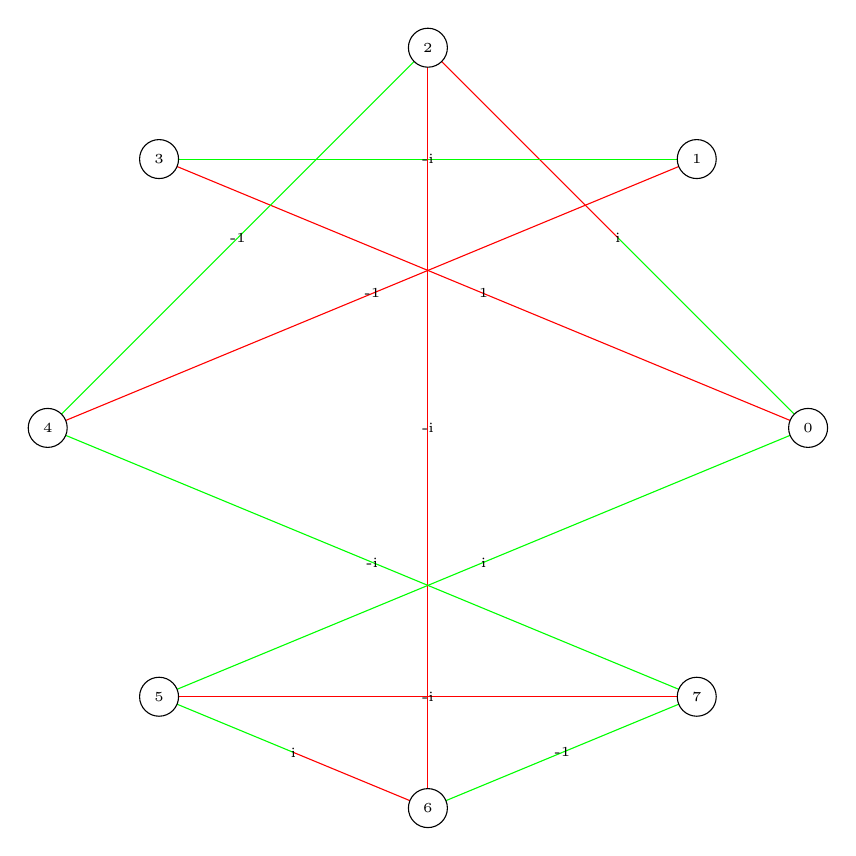
\begin{tikzpicture}
    \tikzstyle{every node}=[font=\tiny]
        \draw [style=thin, color=green] (4.82842712474619,0.0) to (2.414213562373095,2.414213562373095);
        \draw [style=thin, color=red] (2.414213562373095,2.414213562373095) to (2.9565589116183395e-16,4.82842712474619);
        \node [style=circle, draw=none] at (2.414213562373095,2.414213562373095) {i};
        \draw [style=thin, color=red] (4.82842712474619,0.0) to (0.7071067811865477,1.7071067811865475);
        \draw [style=thin, color=red] (0.7071067811865477,1.7071067811865475) to (-3.4142135623730945,3.414213562373095);
        \node [style=circle, draw=none] at (0.7071067811865477,1.7071067811865475) {1};
        \draw [style=thin, color=green] (4.82842712474619,0.0) to (0.707106781186547,-1.7071067811865472);
        \draw [style=thin, color=green] (0.707106781186547,-1.7071067811865472) to (-3.414213562373096,-3.4142135623730945);
        \node [style=circle, draw=none] at (0.707106781186547,-1.7071067811865472) {i};
        \draw [style=thin, color=green] (3.414213562373095,3.4142135623730945) to (2.220446049250313e-16,3.414213562373095);
        \draw [style=thin, color=green] (2.220446049250313e-16,3.414213562373095) to (-3.4142135623730945,3.414213562373095);
        \node [style=circle, draw=none] at (2.220446049250313e-16,3.414213562373095) {-i};
        \draw [style=thin, color=red] (3.414213562373095,3.4142135623730945) to (-0.7071067811865475,1.7071067811865475);
        \draw [style=thin, color=red] (-0.7071067811865475,1.7071067811865475) to (-4.82842712474619,5.913117823236679e-16);
        \node [style=circle, draw=none] at (-0.7071067811865475,1.7071067811865475) {-1};
        \draw [style=thin, color=green] (2.9565589116183395e-16,4.82842712474619) to (-2.414213562373095,2.4142135623730954);
        \draw [style=thin, color=green] (-2.414213562373095,2.4142135623730954) to (-4.82842712474619,5.913117823236679e-16);
        \node [style=circle, draw=none] at (-2.414213562373095,2.4142135623730954) {-1};
        \draw [style=thin, color=red] (2.9565589116183395e-16,4.82842712474619) to (-2.9565589116183395e-16,0.0);
        \draw [style=thin, color=red] (-2.9565589116183395e-16,0.0) to (-8.869676734855019e-16,-4.82842712474619);
        \node [style=circle, draw=none] at (-2.9565589116183395e-16,0.0) {-i};
        \draw [style=thin, color=green] (-4.82842712474619,5.913117823236679e-16) to (-0.7071067811865479,-1.7071067811865477);
        \draw [style=thin, color=green] (-0.7071067811865479,-1.7071067811865477) to (3.414213562373094,-3.414213562373096);
        \node [style=circle, draw=none] at (-0.7071067811865479,-1.7071067811865477) {-i};
        \draw [style=thin, color=green] (-3.414213562373096,-3.4142135623730945) to (-1.7071067811865483,-4.121320343559642);
        \draw [style=thin, color=red] (-1.7071067811865483,-4.121320343559642) to (-8.869676734855019e-16,-4.82842712474619);
        \node [style=circle, draw=none] at (-1.7071067811865483,-4.121320343559642) {i};
        \draw [style=thin, color=red] (-3.414213562373096,-3.4142135623730945) to (-8.881784197001252e-16,-3.414213562373095);
        \draw [style=thin, color=red] (-8.881784197001252e-16,-3.414213562373095) to (3.414213562373094,-3.414213562373096);
        \node [style=circle, draw=none] at (-8.881784197001252e-16,-3.414213562373095) {-i};
        \draw [style=thin, color=green] (-8.869676734855019e-16,-4.82842712474619) to (1.7071067811865466,-4.121320343559643);
        \draw [style=thin, color=green] (1.7071067811865466,-4.121320343559643) to (3.414213562373094,-3.414213562373096);
        \node [style=circle, draw=none] at (1.7071067811865466,-4.121320343559643) {-1};
        \node [style=circle, fill=white, draw=black] (0) at (4.82842712474619,0.0) {0};
        \node [style=circle, fill=white, draw=black] (1) at (3.414213562373095,3.4142135623730945) {1};
        \node [style=circle, fill=white, draw=black] (2) at (2.9565589116183395e-16,4.82842712474619) {2};
        \node [style=circle, fill=white, draw=black] (3) at (-3.4142135623730945,3.414213562373095) {3};
        \node [style=circle, fill=white, draw=black] (4) at (-4.82842712474619,5.913117823236679e-16) {4};
        \node [style=circle, fill=white, draw=black] (5) at (-3.414213562373096,-3.4142135623730945) {5};
        \node [style=circle, fill=white, draw=black] (6) at (-8.869676734855019e-16,-4.82842712474619) {6};
        \node [style=circle, fill=white, draw=black] (7) at (3.414213562373094,-3.414213562373096) {7};
    \end{tikzpicture}
    \caption{A perfectly monochromatic graph of size $8$ vertices, with a weighted matching index of $2$, discovered by EGPI during the experiment.}
    \label{fig:egpi_graph_example}
\end{figure}

From the results in figure~\ref{fig:results-experiment}, we can do the following observations.
Firstly, it is a lot harder to find perfectly monochromatic graphs in these conditions when their size is bigger.
Indeed, the number of possibilities grows exponentially with the number of vertices, and the probability to find a perfectly monochromatic graph decreases.
Secondly, the complexity bound has a big impact on the number of found graphs: a higher complexity bound results in a smaller number of found graphs.
This was expected, since the graphs generated with a higher complexity bound have higher chances to have more edges and perfect matchings.
The probability that all these randomly generated edges and perfect matchings together satisfy the definition~\ref{def:perfectly_monochromatic_graph} are small.\\

The last thing I am interested in is to count bipartite graphs among all the perfectly monochromatic graphs found.
The result is the following: \textbf{none} of the perfectly monochromatic graphs found were bipartite.
This is an alluring new observation: indeed, it is consistent with the arguments we used in the proofs of lemmas~\ref{lem:one_neg_edge} and~\ref{lem:2_positive_colour_classes_forbidden}.
One of the observations these proofs used is that, in these particular cases, the perfectly monochromatic graphs found were not bipartite.
This allows me to formulate the following conjecture.

\begin{conjecture}
    \label{con:bipartite_perfectly_monochromatic}
    Let $G_k^w$ be a non-redundant perfectly monochromatic graph that respects the following properties.
    \begin{itemize}
        \item $\Tilde{c}(G, k, w) \geq 2$
        \item $\forall e \in E(G_k^w), w(e) \in \{-1, 1, -i, i\}$
        \item $G_k^w$ has at least one non-monochromatic feasible vertex colouring.
    \end{itemize}
    Then, $G_k^w$ is not bipartite.
\end{conjecture}

This conjecture might constitute a new interesting subcase of the Krenn's conjecture to investigate in the future.


\subsubsection{Possible improvements for EGPI}

EGPI is a tool that can still be improved in many ways.\\

Firstly, currently it does not offer the functionality of generating only non-isomorphic graphs.
This functionality could be interesting if the user wants to count the number of different graphs generated by the tool.
This could be coded from scratch, or by using an external program.
For instance, in Python, the package \textit{NetworkX} offers a function to check if $2$ graphs are isomorphic or not~\cite{networkx}.
A more common program used a lot in the field of graph theory is Nauty, a program originally designed by Brendan McKay~\cite{MCKAY201494}.
Using it would offer a lot of advantages, but it would require to write a wrapper around it to use it in Python.
Indeed, Nauty is written in C. \\

A second improvement that could be brought to EGPI is to improve the efficiency of the algorithms used to find the perfect matchings of a graph.
Indeed, this step bounds the efficiency of most of the tasks performed by EGPI\@.
Improving this algorithm would allow the program to search more graphs in a given time, and to find more results in general.
One idea to improve it could be to look at the Edmonds' Blossom algorithm, an algorithm to find a single perfect matching in a graph~\cite{Edmonds_1965}.
It has to be determined whether this algorithm can be adapted to find all perfect matchings of a graph.\\
